% Options for packages loaded elsewhere
\PassOptionsToPackage{unicode}{hyperref}
\PassOptionsToPackage{hyphens}{url}
\PassOptionsToPackage{dvipsnames,svgnames,x11names}{xcolor}

\documentclass[12pt]{article}

\usepackage{amsmath,amssymb,amsfonts}
\usepackage{bm}
\usepackage{graphicx}
\usepackage{xcolor}
\usepackage{xspace}
\usepackage{xparse}
\usepackage{iftex}
\ifPDFTeX
  \usepackage[T1]{fontenc}
  \usepackage[utf8]{inputenc}
  \usepackage{textcomp}
\else
  \usepackage{unicode-math}
  \defaultfontfeatures{Scale=MatchLowercase}
  \defaultfontfeatures[\rmfamily]{Ligatures=TeX,Scale=1}
\fi
\usepackage{lmodern}
\IfFileExists{upquote.sty}{\usepackage{upquote}}{}
\IfFileExists{microtype.sty}{%
  \usepackage[]{microtype}
  \UseMicrotypeSet[protrusion]{basicmath}
}{}

\setlength{\emergencystretch}{3em}
\setcounter{secnumdepth}{5}

\AtBeginDocument{%
\ifdefined\contentsname
  \renewcommand*\contentsname{Table of contents}
\else
  \newcommand\contentsname{Table of contents}
\fi
\ifdefined\listfigurename
  \renewcommand*\listfigurename{List of Figures}
\else
  \newcommand\listfigurename{List of Figures}
\fi
\ifdefined\listtablename
  \renewcommand*\listtablename{List of Tables}
\else
  \newcommand\listtablename{List of Tables}
\fi
\ifdefined\figurename
  \renewcommand*\figurename{Figure}
\else
  \newcommand\figurename{Figure}
\fi
\ifdefined\tablename
  \renewcommand*\tablename{Table}
\else
  \newcommand\tablename{Table}
\fi
}

\usepackage[]{natbib}
\bibliographystyle{apalike}

\IfFileExists{xurl.sty}{\usepackage{xurl}}{}
\usepackage[
  colorlinks=true,
  breaklinks=true,
  linkcolor=blue,
  anchorcolor=black,
  citecolor=Blue,
  filecolor=Maroon,
  menucolor=red,
  urlcolor=Blue]{hyperref}
\urlstyle{same}
\usepackage{bookmark}

\hypersetup{
  pdftitle={Comments on Deep Fréchet Regression},
  pdfauthor={Edward Gunning; Kyle Stanley; Jeffrey S. Morris; Giles Hooker},
  pdfkeywords={Fréchet regression, object data, manifold learning, deep learning},
  pdfcreator={LaTeX}}

\addtolength{\oddsidemargin}{-.5in}
\addtolength{\evensidemargin}{-.1in}
\addtolength{\textwidth}{1in}
\addtolength{\textheight}{1.7in}
\addtolength{\topmargin}{-1in}
\newcommand{\Frechet}{Fr\'echet\xspace}
\newcommand{\anon}{1}
\let\natbibtextcite\citet
\let\natbibparencite\citep
\NewDocumentCommand{\textcite}{o m}{%
  \IfNoValueTF{#1}{\natbibtextcite{#2}}{\natbibtextcite[#1]{#2}}%
}
\NewDocumentCommand{\parencite}{o o m}{%
  \IfNoValueTF{#1}{%
    \natbibparencite{#3}%
  }{%
    \IfNoValueTF{#2}{\natbibparencite[#1]{#3}}{\natbibparencite[#1][#2]{#3}}%
  }%
}

\begin{document}

\def\spacingset#1{\renewcommand{\baselinestretch}{#1}\small\normalsize}
\spacingset{1}

\if1\anon
{
  \title{\bf Comments on \emph{``Deep \Frechet Regression''} by Su I Iao, Yidong Zhou \& Hans-Georg Müller}
  \author{
    Edward Gunning\hspace{.2cm}\\
    School of Mathematical Sciences,\\ University College Cork, Ireland\\
    and\\
    Kyle Stanley\\
    Department of Biostatistics, Epidemiology and Informatics, \\University of Pennsylvania\\
    and\\
    Jeffrey S. Morris\\
    Department of Biostatistics, Epidemiology and Informatics,\\ University of Pennsylvania\\
    and\\
    Giles Hooker\\
    Department of Statistics and Data Science,\\ University of Pennsylvania}
  \date{September 2026}
  \maketitle
} \fi

\if0\anon
{
  \bigskip
  \bigskip
  \bigskip
  \begin{center}
    {\LARGE\bf Comments on \emph{``Deep \Frechet Regression''}}
  \end{center}
  \medskip
} \fi

\bigskip
\begin{abstract}
We provide a written commentary of the article \emph{Deep Fr\'echet Regression} by \textcite{iao_deep_2025}, which was presented at the JASA Theory and Methods Invited Session at the 2026 Joint Statistical Meetings (JSM).
\end{abstract}

% \noindent%\input{jasa-manuscript}
% {\it Keywords:} Fréchet regression, object data, manifold learning, deep learning
\vfill

\newpage
\spacingset{1.8}

\section{Introduction}

We congratulate the authors on an important contribution which further enriches a general and substantive program on modeling complex object responses using \Frechet methods, emanating from the seminal work of \textcite{petersen_frechet_2019}.
In recent years, there has been an increase in the volume, complexity and diversity of data objects being collected.
Many of these modern object types have non-Euclidean, complex high-dimensional structure, e.g., networks \parencite{desai_connectivity_2023, zhou_network_2022}, probability distributions \parencite{kneip_inference_2001,petersen_functional_2016, yang_quantile_2020}, shapes \parencite{wu_shape-based_2024}, and brain cortical surfaces \parencite{Chung2022BrainSurfaces}.
The development of principled statistical approaches that leverage the objects' inherent structure and obey their geometric constraints is a very important endeavor.
Moreover, we are glad to see the authors combine modern deep-learning methods within classical statistical approaches, thereby developing a ``hybrid'' framework that benefits from the strengths of both strategies.




We appreciate the generality of the mathematical results that this approach allows. However, that generality also leaves a significant amount of detail that must be specified for any particular study.
Here we consider some issues regarding the practical implementation of the DFR framework that we believe are worthy of further discussion.

\section{Selecting the Intrinsic Manifold Dimension}

The authors employ the ISOMAP technique as the default dimension reduction method in both their manuscript and code\footnote{\href{https://github.com/SUIIAO/Deep-Frechet-Regression}{https://github.com/SUIIAO/Deep-Frechet-Regression}}, though their network data application employs Multidimensional Scaling (MDS) to represent the graph Laplacian objects.
The dimension of the latent embedding space, which the authors denote by $r$, is fixed at $r=2$ for all three examples---the distributional simulation study, the traffic networks example, and the mortality distributions application in the supplementary material---and the current software implementation only permits $r\leq2$.
For the simulation study, $r=2$ is appropriate by construction.
Still, this true intrinsic dimension would not be known \emph{a priori} in a real data analysis setting.
More generally, it is not clear whether it will always be a sensible default, nor whether the methodology is sensitive to mis-specification of this dimension.

This dimension reduction step plays a crucial role in the proposed methodology.
The low-dimensional latent Euclidean embeddings are treated as surrogates for the original objects, allowing them to be regressed non-parametrically on Euclidean predictors using deep learning.
The fitted values from this regression are then used as predictors within local \Frechet regression.
Motivated in this way, it seems reasonable that an effective dimension reduction method should have two main properties.
Firstly, the latent embeddings should preserve all (or most) of the structure in the original object space, such that the relationship with the predictors can be faithfully captured in the non-parametric regression.
Second, since the fitted embeddings are used as predictors in the \Frechet regression step, they should be as low-dimensional as possible, to avoid the curse of dimensionality in local regression, which is captured by the derived convergence rate for multivariable local \Frechet regression in Proposition 1 of the manuscript.
In our own work \parencite[Compact near-Lossless Latent Representations (CLaRe);][]{zohner_clare_2025}, we call these two properties \textbf{(near-)losslessness} and \textbf{compactness}.
In practice, they can be regulated through the dimension reduction method and the dimension of the lower-dimensional embedding space ($r$).

Due to the general metric structure, DFR employs non-invertible manifold learning techniques for dimension reduction that require only a pairwise distance matrix between observations (e.g., ISOMAP, MDS).
In contrast, CLaRe focuses on dimension reduction methods with explicit encoding-decoding architectures.
We use the generalization error of decoded objects to measure the degree to which their structure is captured.
For non-invertible manifold learning techniques, an analogue might be how well the objects' geodesic distances are preserved by the lower-dimensional embeddings.
In CLaRe we argue that to confidently use the embeddings as surrogates for the individual objects in downstream analysis, we should aim to control (out-of-sample) individual observation-level reconstruction error, rather than aggregated measures.
In the manifold learning context, one might examine the geodesic distance reconstructions for each object individually, rather than aggregate them over the whole dataset, although we must assume some further structure to translate this into lossless reconstruction of the original data objects.

To translate our point on manifold dimension selection into a practical example, we have built on the authors' simulation scenario from the main paper and supplementary material.
We simulated a dataset of size $n=500$ from their original Gaussian data setting and from their perturbed Gaussian setting, using these as references.
We then simulated a dataset in the same way from a \emph{skew-normal} distribution, parameterized such that the random means and variances of each distribution are drawn from the same common population distributions as in the authors' examples, but these new random distributions additionally depend on a skew parameter $\alpha$ \parencite{azzalini_skew-normal_2013}.
The conditional expectation of the $\alpha$ parameter was generated as a non-linear function of the generated covariates, such that it had a non-linear relationship with the expected mean and variance. 
We also interacted it with the binary covariate $X_9$, so that it could reflect a realistic group effect.

The top row of Figure \ref{fig:simulation-example} displays the three datasets, represented in terms of their discretized empirical quantile functions.
On the surface, all three sets of discretized empirical quantile functions appear reasonably similar and it is not immediately obvious that $r>2$ might be required for the third dataset, but not for the first and second.
The second row of Figure \ref{fig:simulation-example} shows a linear projection of the discretized quantile functions onto three dimensions that approximately represent the mean, variance, and skewness of the distributions, respectively, colored according to the feature $X_9$.
Here, the difference in dimensionality is more evident---for the skew-normal example, there is additional structured variation in the skewness (vertical) coordinate, exhibiting a between-group/covariate dependence.
The third and fourth rows display some diagnostics that could be used to identify a suitable ISOMAP manifold dimension, $r$.
The third row displays the first ten eigenvalues from the classical multidimensional-scaling step inside ISOMAP; we interpret these as an aggregated measure of how well an $r$-dimensional ISOMAP representation preserves the geodesic distances in the dataset.
More in line with our CLaRe philosophy, in the bottom row (left) we present a measure of how well each of the $500$ observations' geodesic distances with the other objects is preserved in the skew-normal example, for $r=1, \dots, 4$. 
This plot makes it clearer that $3$ dimensions should be retained with ISOMAP to preserve the structure in the original space, since the distance reconstruction errors almost vanish when moving from a two to three-dimensional representation. 
Finally, on the right of the bottom panel, we plot the third ISOMAP dimension against the true expected $\alpha$ parameter; very clearly, this dimension is required for capturing the between-group difference.

This short example demonstrates that careful selection of the embedding dimension $r$ is an important step of the DFR methodology and should be given further consideration.
When such an investigation finds that $r \gg 2$ is required, as we have found in different scientific applications, some guidance on whether DFR is still feasible or whether alternatives need to be considered could be provided.

\begin{figure}
    \centering
    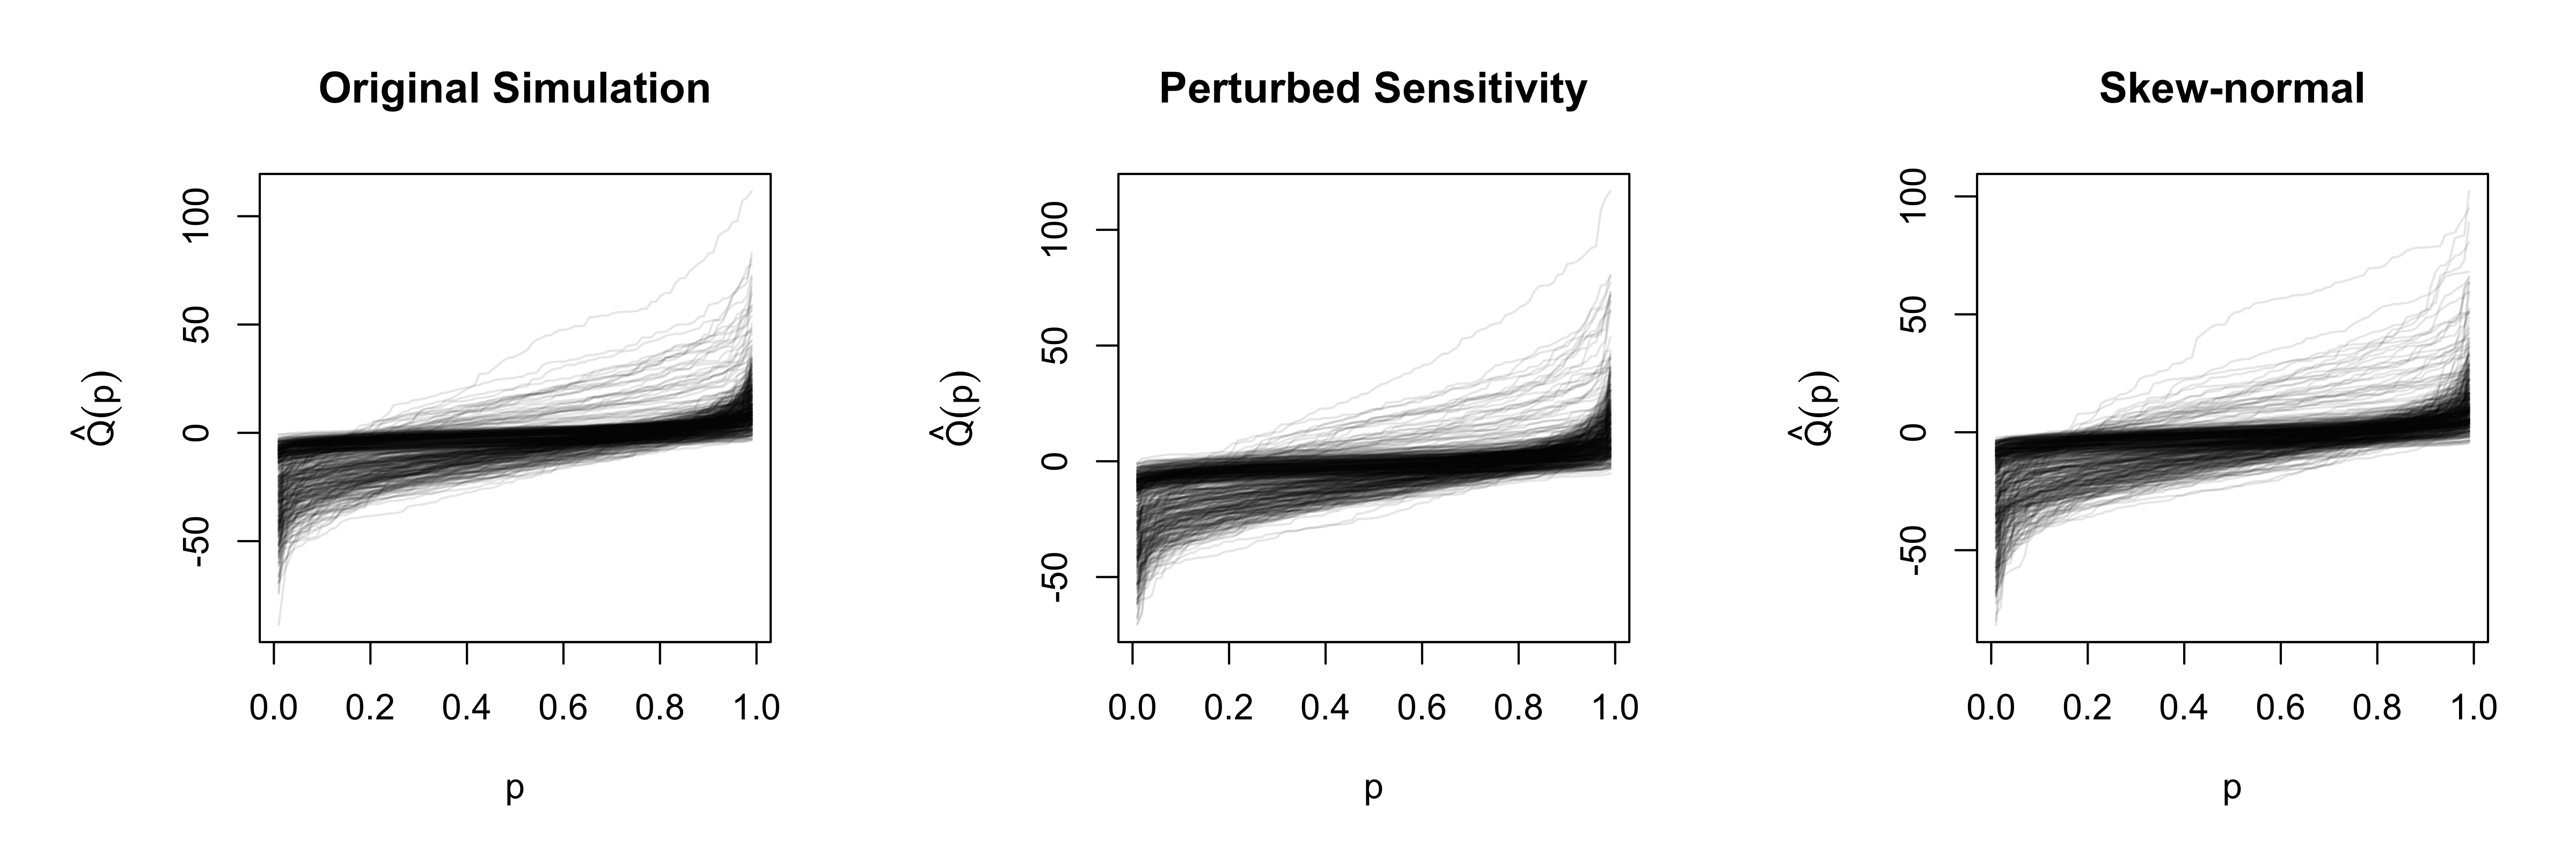
\includegraphics[width=0.7\linewidth]{figures/qfs-group-third-isomap.png}
    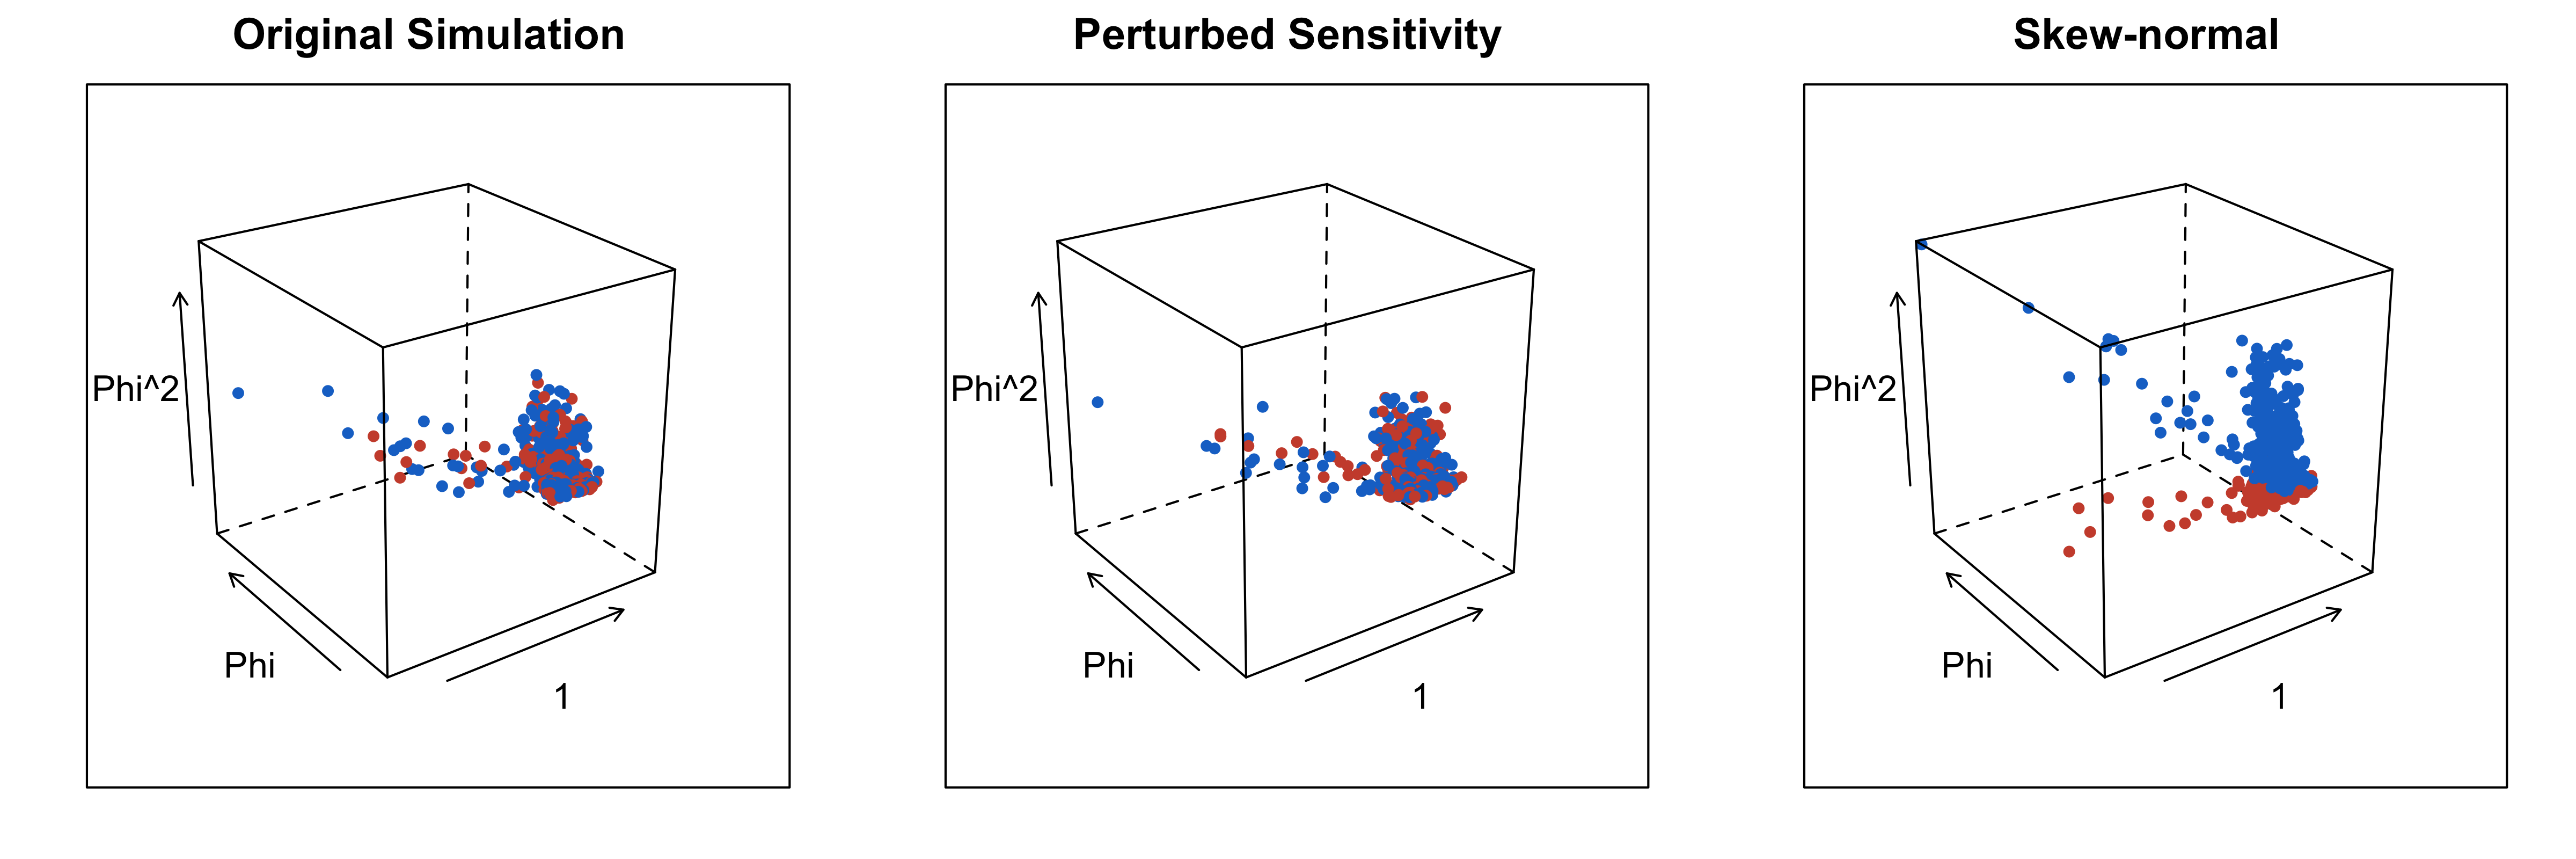
\includegraphics[width=0.75\linewidth]{figures/manifold-data-group-third-isomap.png}
    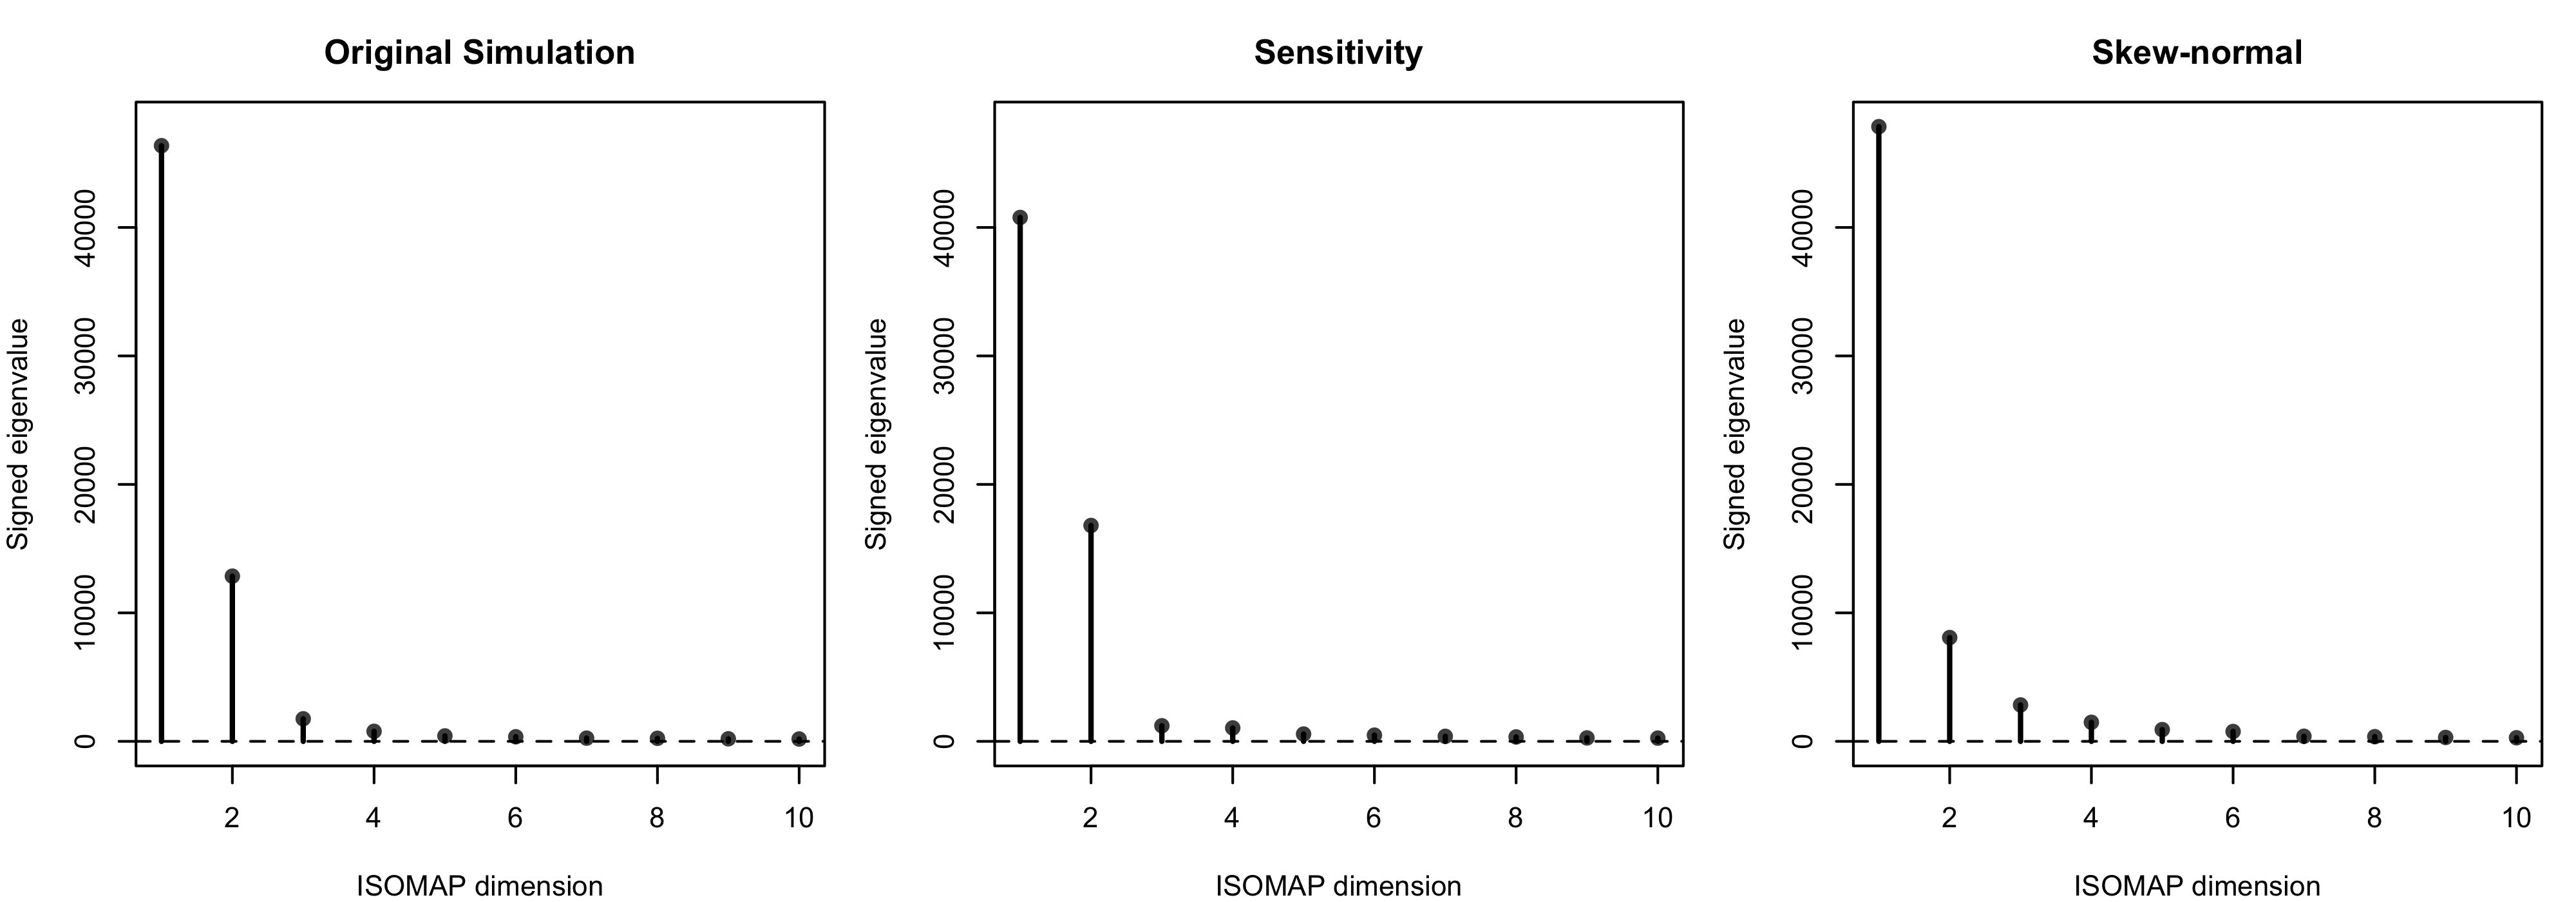
\includegraphics[width=0.675\linewidth]{figures/isomap-eigenvalues-group-third-isomap.png}
    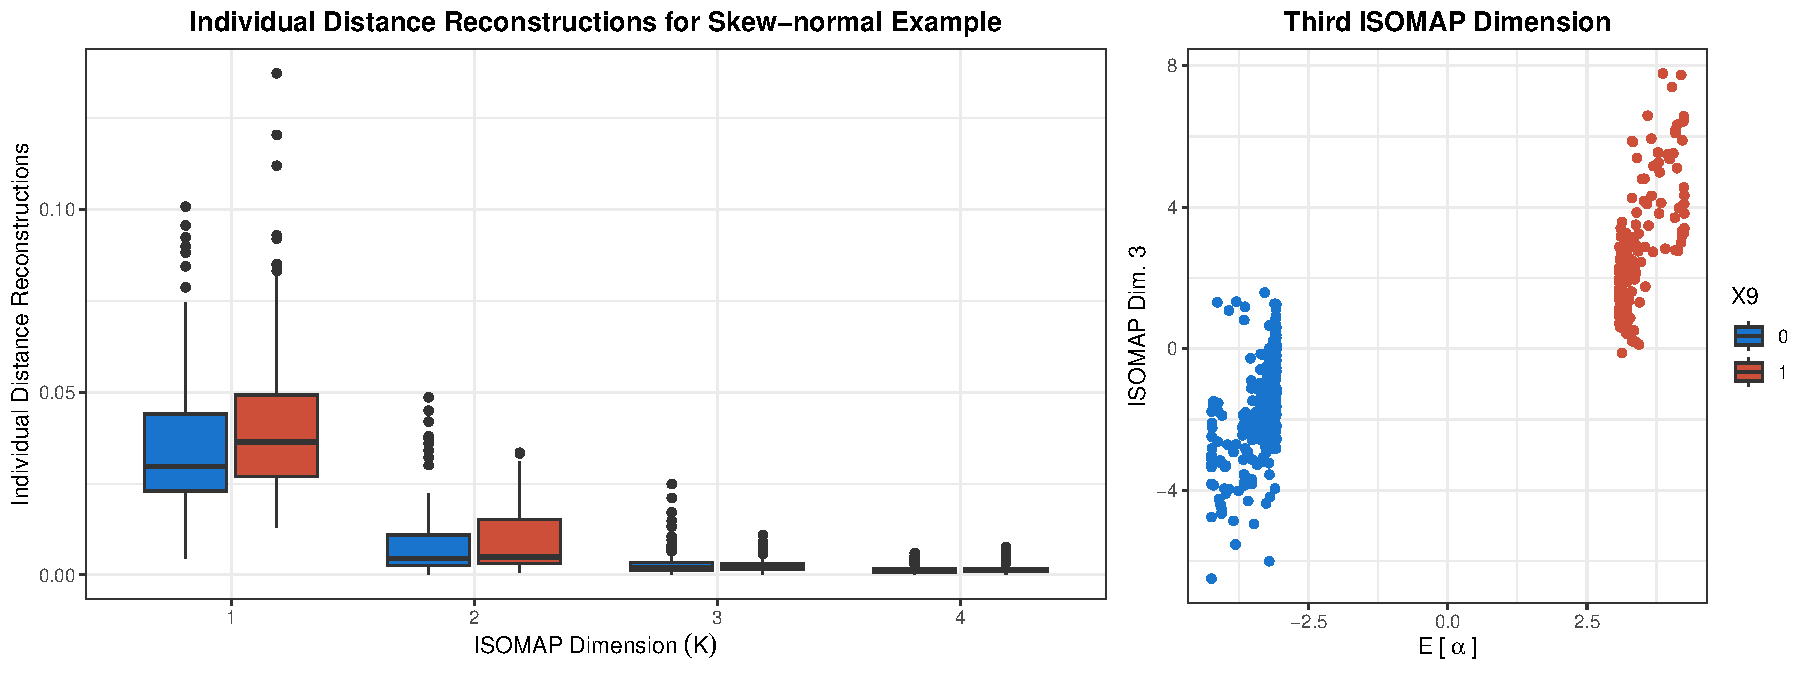
\includegraphics[width=0.7\linewidth]{figures/bottom-row-plot.pdf}
    \caption{
    \small
    \textbf{First row}: The empirical quantile functions from the authors' main simulation, their sensitivity analysis and our skew-normal example (left, center and right, respectively).
    \textbf{Second row}: A linear projection of the empirical quantile functions into three-dimensional space that approximately spans the skew-normal family for each of the examples.
    Points are colored according to their value of the binary covariate $X_9$.
    \textbf{Third row}: The eigenvalues obtained from the classical multidimensional-scaling step inside ISOMAP for each of the examples.
    \textbf{Fourth row}: \textbf{Left}: Boxplot of the individual observations' geodesic distance reconstructions as a function of the ISOMAP dimension $r$, stratified by the binary covariate $X_9$.
    \textbf{Right}: The third ISOMAP coordinate plotted against the true expected $\alpha$ skewness parameter, colored according to $X_9$.
    }
    \label{fig:simulation-example}
\end{figure}

\section{Does Generality Preclude Decoders?}

The CLaRe framework assumes both an encoder and a decoder in order to assess reconstruction error. Local \Frechet regression maps to an encoder, but not in reverse. This yields a model in which errors appear both in the latent and the object space. One of the attractive features of DFR is that it only requires the response objects to live in a space equipped with a metric.
In practice, however, computation of the local \Frechet regression model involves a search over the space of objects (the paper's (14)), which implies the need for additional structure.
Structure, in this context, refers to how the objects are represented numerically in a vector (i.e., ``vectorized'') in order to perform computations.
Object-specific examples include the discretized quantile function representation of distributions and the positive semidefinite matrix parametrization of covariance objects.

Once a vectorization structure for the objects has been assumed, we are back to working within a constrained subset of Euclidean space, where explicit encoder-decoder architectures could be applied.
On a case-by-case basis, we can often find a transformation that maps the vectorized representations to unconstrained Euclidean space, e.g., the log-quantile density transformation for quantile functions \parencite{petersen_functional_2016} and the multivariate generalization of Fisher’s transformation for correlation matrices \parencite{desai_connectivity_2023}.
Such transformations can be used to compose bespoke encoder-decoder architectures for different object types, at the expense of the full generality that DFR provides.

The advantage of employing a transformation that decodes objects is that it allows us to eliminate, reduce, or at least diagnose approximation error in the latent space due to object reconstruction, isolating error purely from the latent non-parametric model.
At present, DFR has approximation error from both sources, and although it is accounted for in the authors' theory, it can be challenging to assess in practice, as highlighted in the skew-normal example above. 
In our own framework that is applied to images \parencite{gunning2026statistical}, we employ a near-lossless encoder-decoder architecture and a parametric latent regression model.
Doing so constrains approximation error to the familiar Euclidean setting, where classical assessments and diagnostics can be employed.
It is useful to contrast this with subsequent developments to the \Frechet regression framework, where the dual error source is eliminated by applying deep learning directly to learn the regression weights \parencite{zhou_end--end_2026}. These still require a case-by-case instantiation of a local search, usually harnessing additional vectorization that would also admit a decoder architecture.

\section{Conclusion}

The authors are to be congratulated on developing a very general strategy for regressing complex object data on Euclidean predictors. 
The main strength of the methodology is its generality and flexibility, imposing minimal assumptions on the object-valued responses and the effects of covariates. 
It is supported by strong theoretical results and exemplified using an interesting application to traffic network data.
We believe that the practical applicability of the method could be improved by guidance on selecting the dimension reduction architecture and the intrinsic manifold dimension, for which we have shared some perspectives from our own work employing conventional encoder-decoder architectures.
We also envision that some consideration of inference, scalability and stability, within the context of concurrent developments in the general \Frechet regression program, will further enhance its impact.

\begin{description}
\item[Reproducibility:]
Code to reproduce the example in this manuscript is available at \href{https://github.com/edwardgunning/DFR-JASA-Discussion}{https://github.com/edwardgunning/DFR-JASA-Discussion}.
\vspace{-0.5em}
\item[Generative AI:]
ChatGPT 5.5. was used for coding assistance, copy-editing, and proofreading. Any AI-suggested changes were reviewed and approved manually.
\end{description}

\vskip-2em

\bibliography{references}

\end{document}
